%%%%%%%%%%%%%%%%%%%%%%%%%%%%%%%%%%%%%%%%%
%  Telemac Documentation
%  Example of the TelemacDoc class
%
%%%%%%%%%%%%%%%%%%%%%%%%%%%%%%%%%%%%%%%%%

%----------------------------------------------------------------------------------------
%	PACKAGES AND OTHER DOCUMENT CONFIGURATIONS
%----------------------------------------------------------------------------------------
\documentclass[Stbtel]{../../data/TelemacDoc} % Default font size and left-justified equations
%\documentclass[Telemac2D,french]{TelemacDoc} % Default font size and left-justified equations in french

\begin{document}

\let\cleardoublepage\clearpage

%----------------------------------------------------------------------------------------
%	TITLE PAGE
%----------------------------------------------------------------------------------------
\title{Stbtel}
\subtitle{User Manual}
\version{7.2}
\author{Otto Mattic}
\date{\today}
\maketitle
\clearpage


%----------------------------------------------------------------------------------------
%	COPYRIGHT PAGE
%----------------------------------------------------------------------------------------

\newpage

\thispagestyle{empty}

\TelemacCopyright{}


%----------------------------------------------------------------------------------------
%	TABLE OF CONTENTS
%----------------------------------------------------------------------------------------


\pagestyle{empty} % No headers

\tableofcontents% Print the table of contents itself

%\cleardoublepage % Forces the first chapter to start on an odd page so it's on the right

\pagestyle{fancy} % Print headers again

%----------------------------------------------------------------------------------------
%	The whole thing
%----------------------------------------------------------------------------------------
\chapter{Introduction}
%-------------------------------------------------------------------------------
\section{Presentation of the \stbtel software}
%-------------------------------------------------------------------------------
%
when a model is constructing with the \telemacsystem, the mesh computation is
an important step. Most of the time, this operation is done with the integrated
mesh generator MATISSSE; however, the \telemacsystem allows the interface with
some other mesh generator software. So, the aim of the \stbtel software is to
realise this interface within the \telemacsystem software. Moreover, it permits
also a lot of operations on these meshes:
\begin{itemize}
\item Check of the geometry
\item Interpolation of the bathymetric points
\item Dry elements elimination when using a \telemac{2} results file
\item Mesh extraction
\end{itemize}
Mesh files of the following list are interfaced with the \stbtel version 4.1:
\begin{itemize}
\item The SIMAIL manufactured by SIMULOG.
\item The I-DEAS manufactured by SDRC
\item The TRIGRID program developed by the Institute of Ocean Sciences, Canada
\item The FASTTABS program developed by the Brigham Young University, USA
\end{itemize}
Of course, standard format file of the \telemacsystem (Selafin) can be used by
\stbtel.\\
\stbtel was developed by the National Hydraulics Laboratory (Laboratoire
National d’Hydraulique-LNH) of the Research and Studies Directorate of the
French Electricity Board (EDF-DER). Like previous versions of the program,
version 4.1 complies with EDF-DER’s Quality Assurance procedures for scientific
and technical programs. This sets out rules for developing and checking product
quality at all stages. In particular, a program covered by Quality Assurance
procedures is accompanied by a Formulation Document [01] that describes the
theoretical aspects of the software, and a Validation Document [02] that
describes the validation domain of the software and a set of test cases. This
latter document can be used to determine the performance and limitations of the
software and define its field of application. The test cases are also used for
developing the software and are checked each time new versions that are
produced.

%-------------------------------------------------------------------------------
\section{Situation of \stbtel software within the \telemacsystem modelling system}
%-------------------------------------------------------------------------------

The \stbtel software is part of a complete set of computational software and
their associated pre- and post-processors, the \telemacsystem. This offers all
the modules required for 2D and 3D numerical simulations in hydrodynamics
(currents and waves), sedimentology and water quality.\\
%
\begin{figure}[H]%
\begin{center}
%
  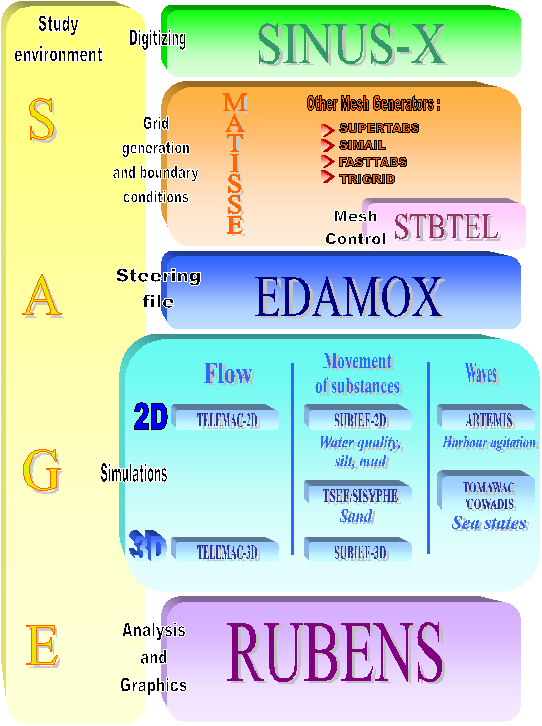
\includegraphics[width=0.9\textwidth]{./graphics/orga}
%
\end{center}
\caption
{Organisation of the modules.}
\label{fig:orga}
\end{figure}

The \telemacsystem, illustrated on figure \ref{fig:orga}, consists of the following
modules:
\begin{itemize}
\item The SINUSX [03] software. This is used, in conjunction with a digitising
pad, to acquire bed data and the limits of the domain that is to be simulated
with the model. The mesh generator will then read the corresponding file.
\item The MATISSE [04] software. This is used to build the grid based on
triangular elements, using the bathymetry.
\item The \stbtel software. This is used, reading the file produced by the mesh
generator, for interpolating bathymetric data (optionally) and creating a
geometry file to the Selafin standard that can be read by the simulation
modules and by the RUBENS graphical post-processor. \stbtel also carries out a
number of mesh consistency checks. Its use is described in this manual.
\item The \telemac{2} [05] software. This carries out the hydrodynamic
simulation. \telemac{2} is also able to simulate the transport of dissolved
tracers.
\item The EDAMOX [06] software. This enables interactive creation of the
steering files required for the various simulation modules.
\item The SUBIEF [07] software. This is used to simulate water quality
phenomena (calculation of the transport by advection/dispersion of dissolved
substances without buoyancy effects) and the transport of suspended sediments.
\item The \sisyphe [08] software. This is used to simulate the transport of bed
load (\sisyphe supersedes the TSEF software within the \telemacsystem)
\item The \artemis [09] software. This computes the transformation of wave
characteristics in a coastal area or harbour.
\item The \telemac{3} [10] software which computes 3D hydrodynamics.
\telemac{3} is also able to simulate the transport of dissolved tracers.
\item The \postel [11] software which produces 2D cuts inside the 3D results
file of \telemac{3}, in order to use the RUBENS graphical post-processor.
\item The RUBENS [12] software. This is used for interactively exploiting and
producing graphical outputs of the results of the various simulation modules.
\item The SAGE software which offers help for the studies management.
\end{itemize}

%-------------------------------------------------------------------------------
\section{Computer environment}
%-------------------------------------------------------------------------------

The simulation modules are written in FORTRAN-77, with no machine-specific
language extensions. A shift to FORTRAN-90 is in progress. They can be run on
all workstations operating under UNIX and on certain vector computers (in
particular Cray and Fujitsu). At EDF-DER, these programs were developed on a
Cray vector computer operating under Unicos and on a HP 9000 series 700
workstation operating under HP-UX.\\
The graphics modules (SINUSX, RUBENS, EDAMOX and MATISSE) can be run on a
workstation operating under UNIX with access to X\_Windows X11R5 and OSF/Motif
libraries


%--------------------------------------------------------------------------------
\chapter{Inputs and outputs}
%--------------------------------------------------------------------------------
%--------------------------------------------------------------------------------
\section{Preliminary remarks}
%--------------------------------------------------------------------------------
During a computation, the \stbtel software uses a number of input and output
files. Some of them are optional.\\
The input files are the following:
\begin{itemize}
\item The steering file,
\item The file containing the mesh to be treated (universal file),
\item One or many bottom topography files,
\item The Fortran file,
\item The optional data file.
The output files are the following:
\end{itemize}
\begin{itemize}
\item The geometry file according to the TELEMAC standard (Selafin)
\item The listing printout,
\item The boundary conditions file.
\end{itemize}

%--------------------------------------------------------------------------------
\section{The files}
%--------------------------------------------------------------------------------
%--------------------------------------------------------------------------------
\subsection{The steering file}
%--------------------------------------------------------------------------------
This is a text file created by the EDAMOX module or directly by the text
editor. In a way, it represents the control panel of the computation. It
contains a number of keywords to which values are assigned. If a keyword is not
contained in this file, \stbtel will assign it the default value defined in the
dictionary file (see description in section 2.2.9). If such a default value is
not defined in the dictionary file, the computation will stop with an error
message. For example, the command MESH = TRIGRID. enables the user to specify
that the computed file comes from the TRIGRID software.\\
\stbtel reads the steering file at the beginning of the computation.\\
The dictionary file and steering file are read by a utility called \damo,
which is included in \stbtel. Because of this, when the steering file is being
created, it is necessary to comply with the rules of syntax used in \damo
(this is done automatically if the file is created with EDAMOX). They are
briefly described below and an example is given in Appendix 4.\\

The rules of syntax are the following:
\begin{itemize}
\item The keywords may be of Integer, Real, Logical or Character type.
\item The order of keywords in the steering file is of no importance.
\item Each line is limited to 72 characters. However, it is possible to pass
from one line to the next as often as required, provided that the name of the
keyword is not split between two lines.
\item For keywords of the array type (only one-dimensional arrays are
available), the separator between two values is the semi-colon. It is not
necessary to give a number of values equal to the size of the array. In this
case, \damo returns the number of read values. For example:
\begin{lstlisting}[language=TelemacCas]
ABSCISSAE OF THE VERTICES OF THE POLYGON TO EXTRACT THE MESH  = 100.5; 500.6
\end{lstlisting}
  (This keyword is declared as an array of 9 values)
\item The signs ":" or "=" can be used indiscriminately as separator for the
name of a keyword and its value. They may be preceded or followed by any number
of spaces. The value itself may appear on the next line. For example:
\begin{lstlisting}[language=TelemacCas]
BOTTOM CORRECTION OF TRIGRID = 10.
\end{lstlisting}
or
\begin{lstlisting}[language=TelemacCas]
BOTTOM CORRECTION OF TRIGRID : 10.
\end{lstlisting}
or again
\begin{lstlisting}[language=TelemacCas]
BOTTOM CORRECTION OF TRIGRID  = 10.
\end{lstlisting}
\item Characters between two "/" on a line are considered as comments.
Similarly, characters between a "/" and the end of line are also considered as
comments. For example:
\begin{lstlisting}[language=TelemacCas]
BOTTOM CORRECTION OF TRIGRID = 280     / Bathy 1
\end{lstlisting}
\item A line beginning with "/" is considered to be all comment, even if there
is another "/" in the line. For example:
\begin{lstlisting}[language=TelemacCas]
      / The geometry file is ./mesh/geo
\end{lstlisting}
\item When writing integers, do not exceed the maximum size permitted by the
computer (for a computer with 32-bit architecture, the extreme values are -2
147 483 647 to + 2 147 483 648. Do not leave any space between the sign
(optional for the +) and number. A full stop is allowed at the end of a number.
\item When writing real numbers, the full stop and comma are accepted as
decimal points, as are E and D formats of FORTAN. ( 1.E-3  0.001  0,001  1.D-3
represent the same value).
\item When writing logical values, the following are acceptable: 1 OUI  YES
.TRUE.  TRUE  VRAI and 0 NON  NO  .FALSE.  FALSE  FAUX.
\end{itemize}
In addition to keywords, a number of instructions or meta-commands interpreted
during sequential reading of the steering file can also be used:
\begin{itemize}
\item Command \telkey{\&FIN} indicates the end of the file (even if the file is not
finished). This means that certain keywords can be deactivated simply by
placing them behind this command in order to reactivate them easily later on.
However, the computation continues.
\item Command \telkey{\&ETA} prints the list of keywords and the value that is assigned
to them when \damo encounters the command. This will be displayed at the
beginning of the listing printout (see section 2.2.7).
\item Command \telkey{\&LIS} prints the list of keywords. This will be displayed at the
beginning of the listing printout (see section 2.2.7).
\item Command \telkey{\&IND} prints a detailed list of keywords. This will be displayed
at the beginning of the listing printout (see section 2.2.7).
\item Command \telkey{\&STO} stops the program and the computation is interrupted.
\end{itemize}
The name of this file is given by using the keyword: \telkey{STEERING FILE}.

%--------------------------------------------------------------------------------
\subsection{The universal file}
%--------------------------------------------------------------------------------
This file holds the mesh to be treated. The software choosen for its creation
will change the format. Sometimes, it could be a file already fomated on the
\telemacsystem standard (Selafin) on which specials computations could be
treated.
In some case, this file could hold bathymetric informations.
The name of the file is given with the keyword: \telkey{UNIVERSAL FILE}

%--------------------------------------------------------------------------------
\subsection{The bottom topography files}
%--------------------------------------------------------------------------------
One of the goals of \stbtel is to interpolate a bathymetry point on the mesh
generator.  So, the bathymetric information must be given in one or in more
SINUSX format data files, or in X, Y Z files.
\stbtel can manage as many as 5 bottom topography files. In this case, it’s
important to take heed of the possible covering up of the zones in each file.
The names of this or these file(s) are given with the keyword: \telkey{BOTTOM
TOPOGRAPHY FILES}.
%--------------------------------------------------------------------------------
\subsection{The fortran user file}
%--------------------------------------------------------------------------------
As every TELEMAC simulation modules, \stbtel uses a Fortan user file.  With
\stbtel, It contains the main program. The role of this main program is simply
to determine the language used for writing the messages (English or French) and
to define the memory space by giving the size values for tables A (real) and IA
(integer).
If the size indicated by the user is too small, the \stbtel run is interrupted
and the software prints the minimum value to be put in the main program on the
listing printout. In the opposite case, the user recovers the exact size used
by the program, so that he can define the memory spaces as accurately as
possible, thus saving CPU memory.
This file is compiled and linked so as to generate the executable program for
the simulation.
The name of this file is given with the keyword: \telkey{FORTRAN FILE}.
An example of a FORTRAN file is given in appendix 5.
%--------------------------------------------------------------------------------
\subsection{The additional file of the mesh generator}
%--------------------------------------------------------------------------------
If there is an interface with the TRIGRID software, the file contains the
connectivity table necessary for the use of \stbtel.
If there is an interface with the FASTTBABS software, this file (which is
therefore optional) holds information about the type of the boundary
conditions.
The name of this file is given with the keyword: \telkey{MESH ADDITIONAL DATA
FILE}.
%--------------------------------------------------------------------------------
\subsection{The geometry file}
%--------------------------------------------------------------------------------
This geometry file is created by \stbtel from the universal file. This file is
done on the TELEMAC standard format (Selafin). It holds the information about
the geometry of the mesh, and possibly bathymetry information.
It’s a binary file that can be used with the RUBENS.
The name of this file is given with the keyword: \telkey{GEOMETRY FILE FOR TELEMAC}.

%--------------------------------------------------------------------------------
\subsection{The listing printout}
%--------------------------------------------------------------------------------
This is an \stbtel running report in which the user can find information about
operations performed by \stbtel.
The name of this file is managed directly by the \stbtel start-up procedure. In
general, it has the name of the steering file associated with the suffix
.sortie. A short example of a listing printout is given in appendix 6.
%--------------------------------------------------------------------------------
\subsection{The boundary conditions file}
%--------------------------------------------------------------------------------
This is a file generated by \stbtel. It can be modified using a text editor.
Each line of this file is dedicated at one point of the boundary. The numbering
of the boundary points is the same as the lines of the file.  It describes
first of all, the contour of the domain in a trigonometric direction from the
bottom left side point (minimum X +Y), then the islands on the clock wise.
For complete description of this file, see the \telemac{2} user manual.
If a mesh is being read with the Selafin format, the boundary conditions file
is not accurately completed by \stbtel (all the points are identified as walls
with slippery conditions).
The name of this file is given with the keyword: \telkey{BOUNDARY CONDITIONS
FILE}.
%--------------------------------------------------------------------------------
\subsection{The dictionary file}
%--------------------------------------------------------------------------------
This file contains all information on the keywords (name in French, name in
English, default values, type, documentation on keywords, information required
by EDAMOX). This file can be consulted by the user but must under no
circumstances be modified.
%--------------------------------------------------------------------------------
\subsection{The libraries}
%--------------------------------------------------------------------------------
When a computation is initiated, the main program written by the user is
compiled and then linked in order to generate the executable that is then run.
During the link edition phase, the following libraries are used:
\begin{itemize}
\item \stbtel: this library contains the subroutines that are specific to the
\stbtel code.
\item util: this library contains a number of utility subroutines, such as, for
example, the file read and writes routines.
\item damo: this library contains all subroutines that manage the reading of
keywords.
\item hp: this library contains the subroutines that manage the writing of the
various binaries (see section 2.3).
\end{itemize}
Usually, the user does not use other libraries than the standard ones. However,
the keyword LIBRARY is implemented to identify the used libraries on the
program generated. (see references manual for more details).
Moreover, the use of the last version installed on the computer is planned on
the software outline. The keyword RELEASE helps to identify the used library
version (for example to initiate a computation using a previous software
version). This keyword is described on the reference manual.
%--------------------------------------------------------------------------------
\section{File binaries}
%--------------------------------------------------------------------------------
The binary of a file is the method used by the computer for storing the
information physically on the disk (in contrast to storage in ASCII form, which
is used by the formatted files). \stbtel recognises three types of binary: the
standard binary of the computer on which the user is working, the IBM binary
enabling a file created on an IBM computer to be re-read, and the IEEE binary
that can be used, for example, to generate a file on a Cray OR IBM computer
that can be read by a workstation (provided that the appropriate subroutines
are included when \stbtel is installed on the computer).
The keyword used to fix the binary of the geometry file generated by \stbtel
is: \telkey{BINARY STANDARD}.
The default value specified on the dictionary file is “STD” (default binary of
the computer that is being used)

%--------------------------------------------------------------------------------
\section{Computer environment}
%--------------------------------------------------------------------------------
When using \stbtel on the main computer, the following keywords help to check
on the software computations. (These keywords are defined on the reference
manual).
\begin{itemize}
\item \telkey{KEYWORD}
\item \telkey{ACCOUNT}
\item \telkey{MEMORY SPACE}
\item \telkey{CPU TIME}
\item \telkey{USER}
\end{itemize}

%--------------------------------------------------------------------------------
\chapter{Mesh treatment}
%--------------------------------------------------------------------------------
When the mesh file is being treated, the computation parameters given by the
user help \stbtel to initiate the followong operations:
\begin{itemize}
\item Read of the mesh file and of the connectivity table
\item Mesh extraction (if required by the user)
\item Print of the geometric data on the listing printout
\item Cutting elements in four (if required by the user)
\item Dry elements elimination (if required by the user)
\item The mesh is initialised on the \telemacsystem format (\stbtel check
especially that the local numeration of the nodes is done on the trigonometric
way).
\item Analysis of the boundaries (area outline, islands) and building of the
boundary points table
\item Overstressed elements elimination (if required by the user)
\item Re-numbering of the nodes used for the optimisation of the matrix storage
on the \telemac{2} software (if required by the user)
\item Elimination of backward dependencies (if required by the user)
\item Interpolation of the bathymetry on the mesh
\item Building of the geometry file
\item Building of the boundary conditions file
\end{itemize}

%--------------------------------------------------------------------------------
\section{Initial treatment}
%--------------------------------------------------------------------------------
\stbtel first goal is to read a mesh file that comes from an outer software. In
this case, the user must indicate the name of the file to be read with the
keyword \telkey{UNIVERSAL FILE}, and, with the keyword \telkey{MESH GENERATOR},
indicates also the name of the software used for mesh generation. This keyword
can be selected among the following:
\begin{itemize}
\item SUPERTAB6 (version 6 of  SUPERTAB mesh generator)
\item SUPERTAB4 (version 4 of  SUPERTAB mesh generator)
\item MASTER2 (version 2 of the MASTER-SERIES mesh generator)
\item SIMAIL,
\item SELAFIN
\item TRIGRID,
\item FASTTABS.
\end{itemize}
When using TRIGRID, the file containing the connectivity table (file with a
“triangle” format) must be given through the keyword \telkey{MESH ADDITIONAL
DATA FILE}.\\
Within a mesh, the three nodes of some triangles can be boundary nodes. In this
case, the computation codes can generate wrong results. This type of elements
called overstressed triangles, must be eliminated when the mesh is being
treated. This action is done with the logical keyword \telkey{OVERSTRESSED
TRIANGLES ELIMINATION} and which the default value in NO. This action is done
by \stbtel.\\
It adds a point at the inertia center of the triangle, in order to
create three more elements. Sometimes, this action can generate flat triangles.
In this case, \stbtel can take the decision to swap segments, in clear, to
reverse the cutting of a quadrangle on the other diagonal. (see Figure
\ref{fig:stress} below). A balance sheet of the overstressed elements
elimination is drawn up with the listing printout.

\begin{figure}[H]%
\begin{center}
%
  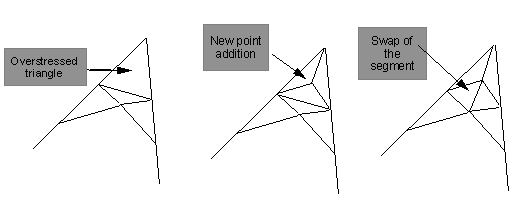
\includegraphics[width=0.9\textwidth]{./graphics/stress}
%
\end{center}
\caption
{Overstressed triangles elimination.}
\label{fig:stress}
\end{figure}


When the mesh is treated, \stbtel allows the elimination of the points that
have a distance value lower at a special value. The user must indicate this
value with the keyword \telkey{MINIMAL DISTANCE BETWEEN TWO POINTS}. This
default value is 0 (no elimination). If the value indicated by the user
eliminates lots of points, \stbtel could be not able to re-build the mesh. In
this case, the computation is automatically interrupted.

%--------------------------------------------------------------------------------
\section{Boundary conditions treatment}
%--------------------------------------------------------------------------------
when a mesh is treated, \stbtel generates automatically the boundary conditions
file.\\
With TRIGRID and SUPERTAB, a colour code stored on the mesh file and associated
with each boundary point permits \stbtel to define the codes to  be generated
within the boundary conditions file (see annexe 10).\\
With FASTTABS, the boundary conditions type can be supply in an additional
file. The user must give the name of this file with the keyword \telkey{MESH
ADDITIONAL DATA FILE} and activate the logical keyword \telkey{BOUNDARY
CONDITIONS IN THE ADDITIONAL FILE}.\\
Then, when using a mesh from SIMAIL software, or from a Selafin file, \stbtel
does not have any information about the type of the boundary conditions. The
generated file assigns with the code “solid boundary” to all the boundary
points.

%--------------------------------------------------------------------------------
\section{Mesh extraction}
%--------------------------------------------------------------------------------
With \stbtel, it is possible to extract a sub-mesh from a global mesh. To
extract one, first of all, the user must choose the polygon that will define
the area of the mesh to be extracted (in the anti clockwise order). This
polygon must have a convex shape.\\
The number of vertices of this polygon must be indicated with the keyword
\telkey{NUMBER OF VERTICES OF THE POLYGON TO EXTRACT THE MESH} and the
coordinates of the points with the keywords \telkey{ABSCISSSAE OF THE VERTICES
OF THE POLYGON TO EXTRACT THE MESH} and  \telkey{ORDINATES OF THE VERTICES OF
THE POLYGON TO EXTRACT THE MESH}.\\
When the mesh is extracted, the user can project new boundaries nodes on the
polygon segments. This action is activated with the logical keyword
\telkey{PROJECTION AFTER EXTRACTION}, with a default value NO.
%--------------------------------------------------------------------------------
\section{Refinement}
%--------------------------------------------------------------------------------
When using \stbtel, a mesh can be refine inside of a zone. To use it, the user
must choose the polygon that will define the area to be refined. As for a mesh
to be extracted, this polygon must have a convex shape and the vertices must be
given with an anti clock wise order. The refinement  generated re-cut the
triangles in four.\\
For the user, the actions to be done are the same than the one used to extract
a mesh.  The number of the vertices of the polygon is given with the keyword
\telkey{NUMBER OF THE VERTICES OF THE POLYGON TO REFINE THE MESH} and the
coordinates of the points with the keyword \telkey{ABSCISSAE OF THE VERTICES OF
THE POLYGON TO REFINE THE MESH} and \telkey{ORDINATES OF THE VERTICES OF THE
POLYGON TO REFINE THE MESH}.
%--------------------------------------------------------------------------------
\section{Special treatments}
%--------------------------------------------------------------------------------
With \stbtel, it is possible to refine the mesh in bulk. This action generates
a new point in the middle of each segments of the triangles. Therefore, each
initial element is cut into four new elements. This action is done with the the
logical keyword \telkey{CUTTING TRIANGLES IN FOUR}, which default value is NO.\\
When using the simulation codes on a vector computer, it is necessary to
foresee the elimination of backward dependencies. This action is done with the
keyword \telkey{ELIMINATION OF THE BACKWARD DEPENDENCIES} and indicates the
length of the vector with the keyword \telkey{VECTOR LENGTH}, with a default
value 1, which means a scalar machine.\\
At least, the use of the assembled elementary storage method for the matrix
storage in \telemac{2} requires a special point numbering that could be done by
\stbtel. This action is completed with the logical keyword \telkey{NODES
RENUMBERING} (default value NO).

%--------------------------------------------------------------------------------
\chapter{Bathymetry treatment}
%--------------------------------------------------------------------------------
The mesh file on \telemacsystem standard can hold a bahymetric information (or
bottom topography) on each point of the mesh. This information can be generated
by \stbtel thanks to two sources:
\begin{itemize}
\item Bottom topography files
\item The mesh generator file itself
\end{itemize}
Furthermore, when the assessment of the memory space necessary for making the
computation is done, \stbtel considers that the number of bathymetric points
does not go beyond 20 000. In the opposite, the user must give the right value
with the keyword \telkey{MAXIMUM NUMBER OF BATHYMETRIC POINTS}.
%--------------------------------------------------------------------------------
\section{Use of the bottom topography files}
%--------------------------------------------------------------------------------
Using any kind of mesh generator  (also while a Selafin file is read), \stbtel
can interpolate on the treated mesh a bathymetry, product of one or more data
files. Their names must be given by the user with the keyword \telkey{BOTTOM
TOPOGRAPHY FILES}. \stbtel can manage five bottom topography files. When using
several files, the user  must  check  the absence of common areas between the
datas or their coherence.\\
Algorithm used by \stbtel to interpolate the bottom topography is the
following: for each mesh point, the space is divided into four quadrants
(depends on the horizontal and vertical). For each quadrant, the software
identifies the nearest bathymetry point, then a balance is done using the found
points. Near the boundary, or, once again, on the island case, it could be
important to ignore the points too close from the boundary. Indeed, the
information found on these points could not be considered. The user is helped
with the keyword \telkey{MINIMUM DISTANCE AT BOUNDARY}. When the mesh point are
interpolated, this keyword dimensions the minimal distance below which a
bathymetry points should be ignored.\\
If the \stbtel informations are too short to interpolate the bathymetry on a
point, the value given to the point is automatically 10-6 m and an error
message is printed on the listing printout.

%--------------------------------------------------------------------------------
\section{Use of the universal file}
%--------------------------------------------------------------------------------
When using a TRIGRID or FASTTABS file, the user can decide to recover in the
mesh file the topography informations . He uses the logical keyword
\telkey{BATHYMETRY ON THE UNIVERSAL FILE} (default value NO).\\
A special information is used with TRIGRID. Indeed, the software works on an
information like "level of water", but not on an information like “bottom
level”. When treating the mesh by \stbtel, it is necessary to restore the
correct bottom elevation value. This computation is done with the help of the
formula: Zf = -Ht + CORR where Zf is the bottom elevation value written by
\stbtel in the geometry file, Ht  the value of the level of water read on the
TRIGRID file, and where CORR  is the user specified value with the keyword
\telkey{BOTTOM CORRECTION OF TRIGRID}. The value of this keyword depends on the
convention chosen by the user when he entered the bathymetric informations in
TRIGRID. Usually, it is the same value used with the utility program \verb!sin2tri!
for the translation of a SINUSX file SINUSX to a TRIGRID file.

\chapter{Dry elements elimination}
when constructing models and during a simulation, (on the fluvial domain for
example, or as for a dam break simulation) it could be well-advised to
eliminate from the mesh the dry elements.\\
It can be realised by \stbtel from the result file of \telemac{2} (or from
others simulation codes producing a result file with the information “level of
water”). It can be activated with the logical keyword \telkey{DRY ELEMENTS
ELIMINATION} (default value NO). \stbtel re-read the entire result file and
determines the nodes mesh that keep dry during the simulation. The user
dimensioned the level of water (in meter) under which we consider that a node
is dry. The user is helped with the keyword \telkey{DRY LIMIT} (default value
0.1). The dry elements are removed of the mesh and the boundaries are re-count
(with island creation if necessary).  By default, only the completely dry
elements are removed (the three triangle points keep dry). In order to remove
completely the dry zones on the domain, the user can specify the partially dry
elements elimination (at least of one dry point) with the keyword
\telkey{PARTIALLY DRY ELEMENTS ELIMINATION} (default value NO)\\
On normal mode, \stbtel stores in the output file only the last time step read
on the \telemac{2} file. The user can ask for the storage of all the time step
with the keyword \telkey{STORAGE OF EVERY TIME STEP} ( default value NO).

\chapter{converter}
%--------------------------------------------------------------------------------
\section{Informations on the formats handled}
%--------------------------------------------------------------------------------

%--------------------------------------------------------------------------------
\subsection{SERAFIN format}
%--------------------------------------------------------------------------------

The SERAFIN format was created for \telemacsystem by EDF. It consists of a binary file
containing the mesh information and the results.  The boundary conditions are
written in an ASCII file or defined in a user's function in \telemacsystem.  What the
file contains is described in the following:

\begin{itemize}
\setlength{\itemsep}{1pt}
\setlength{\parskip}{0pt}
\setlength{\parsep}{0pt}
\item title
\item i,j: number of variables (linear discretization and quadratic
discretization)
\item i+j records of 'name and units of variable' the 16 first characters are
the name and the last 16 are the unit
\item 10 integers: the $7^{th}$ integer gives the number of layers, the
$10^{th}$ indicates that the date is present
\item 4 integers: number of elements (\textit{nelem}), number of points
(\textit{npoin}), number of points defining an element (\textit{ndp}), 1
\item ikles(\textit{npoin}*\textit{ndp}): table of connectivity elements $->$
points
\item ipobo(\textit{npoin}): assigns 1 if the node is a boundary node, 0
otherwise.  If the mesh is distributed ipobo is replaced by
knolg(\textit{npoin}) the local-to-global numbering table
\item x(\textit{npoin}): x coordinates
\item y(\textit{npoin}): y coordinates
\item loop for each time step
\begin{itemize}
\setlength{\itemsep}{1pt}
\setlength{\parskip}{0pt}
\setlength{\parsep}{0pt}
\item The time T (real)
\item loop for each variable \textit{var}
\begin{itemize}
\setlength{\itemsep}{1pt}
\setlength{\parskip}{0pt}
\setlength{\parsep}{0pt}
\item array of \textit{npoin} containing the results for the variable
\textit{var} at time T
\end{itemize}
\item End of the loop on the variables
\end{itemize}
\item End of the loop on the time steps
\end{itemize}

The number of layers is used for \telemac{3} meshes, which is built by extruding the
2D horizontal mesh.  In 3D the z coordinate is the first variable.

The SERAFIN format is used by most of the codes of the \telemacsystem. It can be read
by TECPLOT with the use of a plugin.  The mesh generators Rubens, BlueKenue
and Fudaa PrePro can generate meshes in SERAFIN format.

The pre-\&post-processing tools for parallel simulations, namely
\verb+partel/gretel+, support the SERAFIN format.

Reals are defined in single precision in the SERAFIN format. An identical format
called \textbf{SELAFIND} contains reals in double precision.

%--------------------------------------------------------------------------------
\subsection{MED format}
%--------------------------------------------------------------------------------

The MED3.0.4 format is SALOME's native format. Each MED file is binary.
Information are accessed through the functions of the MED library.

This library is divided in the following sections:

\begin{tabular}{p{70pt}@{ : }p{200pt}p{50pt}}
  \textbf{Library} & Get library informations & mlb* \\
  \textbf{File} & Open/close file & mfi* \\
  \textbf{Profile} & Build selection of nodes & mpf*\\
  \textbf{Mesh} & Information about the mesh (dimension, name, type, coordinates, elements connectivity, \ldots) & mmh*\\
  \textbf{Family} & Read/write of families & mfa*\\
  \textbf{Equivalence} & Link between elements & meq*\\
  \textbf{Joint} & Build a link between two nodes/elements from different partitions (Used for distributed mesh)& msd*\\
  \textbf{Structure} & Creation of new elements & mse*\\
  \textbf{element} & & \\
  \textbf{Field} & Read/write results information & mfd*\\
  \textbf{Link} & Handle link between two meshes & mln*\\
  \textbf{Localization} & Handle element referencing & mlc*\\
  \textbf{Interpolation} & Handle interpolation functions & mip*\\
  \textbf{Parameter} & Read/write constants & mpr*\\
  \textbf{Filter} & Build sub-domains of elements & mfr*\\
\end{tabular}

The library is written mainly in C/C++ but has a Fortran 90 wrapper.
The MED format is used in the \telemacsystem. It can be visualized or modified in SALOME.

%--------------------------------------------------------------------------------
\subsection{UNV format}
%--------------------------------------------------------------------------------

UNV files are ASCII. They are made of a list of sections.

Here is the description of a section:

\begin{itemize}
\setlength{\itemsep}{1pt}
\setlength{\parskip}{0pt}
\setlength{\parsep}{0pt}
\item -1
\item section number
\item \ldots section information \ldots
\item -1
\end{itemize}
In the program we consider 3 sections:
\begin{itemize}
\setlength{\itemsep}{1pt}
\setlength{\parskip}{0pt}
\setlength{\parsep}{0pt}
\item The title section containing the title.
\item The coordinate section containing the coordinates and the color of each
node.
\item The connectivity section containing the connectivity table for the
elements and the color of each element.
\end{itemize}

A complementary ASCII file containing the number of nodes and the total number
of elements also exists (in 3D we can have both 3D and 2D elements).

Note that the UNV format is only used in \estel within the \telemacsystem.
More information about families are also available but they are not used in
\estel.
Most mesh generators can generate meshes in UNV format.
SALOME can read a mesh in UNV format.

%--------------------------------------------------------------------------------
\subsection{VTK format}
%--------------------------------------------------------------------------------

The legacy VTK file format consists of five basic parts:

\begin{enumerate}
\setlength{\itemsep}{1pt}
\setlength{\parskip}{0pt}
\setlength{\parsep}{0pt}
\item The first part is the file version and identifier. This part contains the
single line: \verb+# vtk DataFile Version x.x+.  This line must be exactly as
shown with the exception of the version number x.x, which will change with
different releases of VTK. (Note: the current version number is 3.0. Version
1.0 and 2.0 files are compatible with version 3.0 files).
\item The second part is the header. The header consists of a character string
terminated by the end-of-line character \verb+\n+. The header contains 256
characters at most. It can be used to describe the data and include any other
pertinent information.
\item The third part is the file format. The file format describes the type of
file, either ASCII or binary.  On this line the word 'ASCII' or 'BINARY' has to
be present.
\item The fourth part is the dataset structure. The geometry part describes the
geometry and the topology of the dataset. This part begins with a line
containing the keyword DATASET followed by a keyword describing the type of
dataset.  Then, depending upon the type of dataset, other keyword/data
combinations define the actual data.
\item The final part describes the dataset attributes. This part begins with
the keywords POINT\_DATA or CELL\_DATA, followed by an integer number
specifying the number of points or cells, respectively. (There is no constraint
on the order of appearance of POINT\_DATA or CELL\_DATA). Other keyword/data
combinations then define the actual dataset attribute values i.e., scalars,
vectors, tensors, normals, texture coordinates, or field data.
\end{enumerate}

%--------------------------------------------------------------------------------
\subsection{CGNS format}
%--------------------------------------------------------------------------------

CGNS (CFD General Notation System, latest version 3.1.3) originated in 1994 as
a joint effort between Boeing and NASA, and has since grown to include many
other contributing organizations worldwide. It is an effort to standardize CFD
input and output, including grid (both structured and unstructured), flow
solution, connectivity, boundary conditions, and auxiliary information. CGNS
is also easily extensible, and allows for file-stamping and
user-inserted-commenting. It employs ADF (Advanced Data Format) and/or HDF5
(Hierarchical Data Format) as a database manager which creates binary files
that are portable across computer platforms. It provides a layer of software,
the CGIO Interface which allows access to these database managers at a
low-level, and a second layer of software known as the Mid-Level Library, or
API (Application Programming Interface), which eases the implementation of
CGNS into existing CFD codes.

A CGNS file is an entity that is organized (inside the file itself) into a set
of "nodes" in a tree-like structure, in much the same way as directories are
organized in the UNIX environment.  Strictly speaking, because links may be
used to store information in multiple files, there is no notion of a CGNS
file, only of a CGNS database implemented within one or more files.  However,
throughout this document the two phrases are used interchangeably. The top-most
node is referred to as the "root node." Each node below the root node is
defined by both a name and a label, and may or may not contain information or
data. Each node can also be a "parent" to one or more "child" nodes.  A node
can also have as a child node a link to a node elsewhere in the file or to a
node in a separate CGNS file altogether. Links are transparent to the user:
the user "sees" linked children nodes as if they truly exist in the current
tree. An example of a CGNS tree-like structure is shown below.

\begin{figure} [ht]
\centering
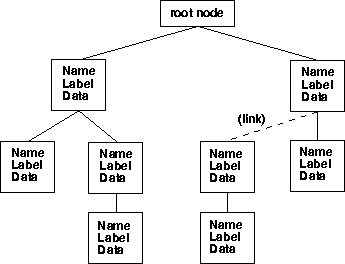
\includegraphics[scale=0.5]{graphics/cgns.png}
\caption{Example CGNS tree-like structure.}
\end{figure}

%--------------------------------------------------------------------------------
\section{\label{upgrades}Description of the new features}
%--------------------------------------------------------------------------------

All the upgrades were included in \stbtel using new parameters, added to the
dictionary. The program still uses the steering file. A parameter determines
whether the new features or the old ones are used.  First are described the new
parameters and features, then will be describe the issues encountered and the
answers given for each format.

%--------------------------------------------------------------------------------
\subsection{Modifications in \stbtel's main program}
%--------------------------------------------------------------------------------

The following table describes the new parameters available for the steering
file:\\

\begin{tabular}{p{140pt}@{ : }p{200pt}}
\textbf{CONVERTER} & (Boolean) If true then use the new features.\\
\textbf{DEBUG} & (Boolean) If true display debug informations.\\
\textbf{SELAFIN IN DOUBLE PRECISION} & (Boolean) If true the SERAFIN file will be read/written in double precision.\\
\textbf{INPUT FILE FORMAT} & (String) The format of the input file, MED, UNV, SERAFIN.\\
\textbf{OUTPUT FILE FORMAT} & (String) The format of the output file, MED, UNV, SERAFIN, VTK.\\
\textbf{INPUT FILE} & (String) The name of the input file.\\
\textbf{BOUNDARY FILE} & (String) The name of the boundary file if it exists (optional).\\
\textbf{LOG FILE} & (String) The name of the complementary file, for the UNV format only.\\
\textbf{OUTPUT FILE} & (String) The name of the output file.\\
\textbf{OUTPUT BOUNDARY FILE} & (String) The name of the output boundary file if it exists (optional).\\
\textbf{OUTPUT LOG FILE} & (String) The name of the output complementary file, for the UNV format only.\\
\end{tabular}

The program works in two steps:
\begin{itemize}
\setlength{\itemsep}{1pt}
\setlength{\parskip}{0pt}
\setlength{\parsep}{0pt}
\item First the file is read and the mesh object structure is filled in.
\item The information from the mesh object structure are written into the
output file.
\end{itemize}

All the format's functions (read/write) are contained in the file
\verb+conv_+\textit{format}\verb+.f+ (where \textit{format} stands for SERAFIN,
MED, \ldots).\\

The table below shows which conversions are possible:

\begin{center}
\begin{tabular}{|l||*{5}{c|}}
\hline
\diagbox{Input}{Output}  & SERAFIN    & MED      & UNV      & CGNS     & VTK    \\
\hline
\hline
SERAFIN     & X         & \checkmark & \checkmark & \checkmark & \checkmark \\
\hline
MED     & \checkmark & X        & \checkmark & \checkmark & \checkmark \\
\hline
UNV     & \checkmark & \checkmark & X        & \checkmark & \checkmark \\
\hline
CGNS    & \checkmark & \checkmark & \checkmark & X        & \checkmark \\
\hline
\end{tabular}\\
\checkmark : Available, X : Unauthorized
\end{center}

The UNV format is the only format that can not manage results. It only
contains the mesh and the colors.

\stbtel handles distributed meshes only for MED and SERAFIN format.

Some formats use a file for each time step for the results file, this is the
case for the VTK format.

Instead of running \stbtel with a steering a script, named \verb+covnerter.py+,
has been created in order to launch the converter in a one-line-command. This
script is written in \textbf{Python 2.6}.

Here is the way it works (To see to following message run \verb+converter.py --help+):
\begin{verbatim}
Usage: converter.py input-file-name -o output-file-name [options]
Example: converter.py coarse.slf -b coarse.cli -o coarse.med --debug
Where coarse.slf is the mesh in SERAFIN fornat,
      coarse.cli is the boundary conditions file and
      coarse.med the converted mesh in MED format.

Options:
  -h, --help            show this help message and exit
  -o OUTPUTFILE, --output-file=OUTPUTFILE
                        name of the output file also defines the
                        output format
  --input-format=INPUTFORMAT
                        name of the input format, overwrites
                         input detected byextension
  --output-format=OUTPUTFORMAT
                        name of the output format, overwrites
                        output detectedby extension
  --output-boundary-file=OUTBOUNDARYFILE
                        name of the output boundary file
  -b BOUNDARYFILE, --boundary-file=BOUNDARYFILE
                        name of the boundary file
  -l LOGFILE, --log-file=LOGFILE
                        name of the log file
  -n NDOMAINS, --ndomains=NDOMAINS
                        number of sub-domains of the distributed mesh
  --srf-bnd             tell stbtel to read the boundary conidtion
                        from theboundary file
  -s, --silent          disable stbtel output informations
  --debug               Enable debug mode which displays more
                        informationsduring run time
  --dx=DX               Value to add to the X coordinates
  --dy=DY               Value to add to the y coordinates
  -r ROOTDIR, --rootdir=ROOTDIR
                        specify the root, default is taken
                        from config file
\end{verbatim}

The conversion of all the files of a distributed mesh in one run is only
available in the python script.

%--------------------------------------------------------------------------------
\subsection{The mesh object structure}
%--------------------------------------------------------------------------------

Here is a description of the object's structure that is used by the converter.
This object makes it easier to add new formats, for each format only two
functions will be needed one to fill the mesh object by reading the file and
one writing the file using the mesh object's data.  A similar object is used in
the \bief library to store mesh information.  This object is used as a common
ground between all the formats handled by the converter.

\begin{description}
\setlength{\itemsep}{1pt}
\setlength{\parskip}{0pt}
\setlength{\parsep}{0pt}
\item[Common Block]
\item[title] Name of the mesh.
\item[description] Description of the mesh (only MED).
\item[ndim] Dimension of the domain (2 or 3).
\item[nelem] Number of elements.
\item[npoin] Number of nodes.
\item[ndp] Number of points per element.
\item[type\_elem] Type of element (triangle, quadrilateral, tetrahedron, prism).
\item[nptfr] Number of boundary nodes.
\item[ib] Table of 10 integers: ib(10) (only used for SERAFIN).
\item[ikles] Connectivity table: ikles(nelem*ndp).
\item[ipobo] Flag for boundary node: ipobo(npoin).
\item[x] x coordinates: x(npoin).
\item[y] y coordinates: y(npoin).
\item[z] z coordinates: z(npoin).
\item[namecoo] Name of the coordinates: namecoo(ndim).
\item[unitcoo] Unit of the coordinates: unitcoo(ndim).
\item[knolg] Global number of point: knolg(npoin).
\item[Results information]
\item[nvar] Total number of variables.
\item[namevar] Name of the variables: namevar(maxvar).
\item[unitvar] Unit of the variables: unitvar(maxvar).
\item[timestep] Number of time steps.
\item[times] Table containing for each time step its value in seconds: times(timestep).
\item[res] Results for all the time steps and all the variables: res(timestep,nvar,npoin).
\item[Families information]
\item[nfam] Number of families.
\item[idfam] id of the family: idfam(nfam).
\item[valfam] Value of each family: valfam(nfam).
\item[namefam] Name of each family: namefam(nfam).
\item[ngroupfam] Number of group of each family: ngroupfam(nfam).
\item[groupfam] Group of each families: groupfam(nfam,10).
\item[Boundary information]
\item[nbor] Local number of each boundary node: nbor(nptfr).
\item[libor] Value of each boundary node: libor(nptfr).
\item[\estel second element type information]
\item[nelem2] Number of elements.
\item[ndp2] Number of points per element.
\item[type\_elem2] Type of element.
\item[ikles2] Connectivity table: ikles2(nelem*ndp).
\item[Color information]
\item[color] Color of a node: color(npoin).
\item[ncolor] Color of an element: ncolor(nelem).
\item[ncolor2] Color of an element (\estel's second element): ncolor2(nelem2).
\end{description}


%--------------------------------------------------------------------------------
\subsection{SERAFIN}
%--------------------------------------------------------------------------------

The code is implemented following the \bief library standards as much as
possible. Three subroutines are used to read the mesh information
\verb+readgeo1+, \verb+readgeo2+, \verb+readgeo3+. But they do not read the
title, the variable information nor the result information. The functions
\verb+lit/ecri2+ of the \bief are used to read and write the extra information.
The \verb+readgeo+ functions contain an optional parameter in order to handle
double precision real.  But in Fortran for the optional parameter to work, a
function has to be declared in an interface and the function in which it is
called must contain the line \verb+use module+ which calls the interface.

When the results part of the SERAFIN file is reached, the results table
(\textbf{res} in mesh object) cannot be allocated because the number of time
steps is unknown at this stage.  To compute this value a quick read trough the
rest of the file is carried out in order to count the number of records.  The
file is then rewound, the results table can now be allocated and filled in.

Because the function rewind causes problems with some machines/compilers (for
instance with GCC-4.1.2) the file is closed and re-opened instead.

An extra file which contains the read/write functions for the boundary file has
been added.

Note that the title is set to have a length of 72 characters in the \bief
library but it is defined with a length of 80 in the TECPLOT plug-in and the
\verb+sel2vtk+ program.

%--------------------------------------------------------------------------------
\subsection{MED}
%--------------------------------------------------------------------------------

Families are used to assign a value to a point. They can also be used to
represent colors or boundary conditions.  A family and a group is created for
each value (\verb?lihbor*100+liubor*10+livbor?). \verb+lihbor+, \verb+liubor+
and \verb+livbor+ are the first three columns of the boundary file.
\verb+hbor+, \verb+ubor+, \verb+vbor+ cannot be stored because they are defined
as floating points whereas the family's value can only be an integer.

As a node only belongs to one family, both color and boundary conditions cannot
be handled.  Currently either color or boundary features are handled, with
priority to the boundary conditions if both are available.

The zero family has to be defined in MED as it is the default family.

MED allows to manipulate vectors (the \verb+ifvector_+ function from
\verb+m_med.f+ in the \bief library defines which variable is a vector). Those
variables are then merged into one. For example the variables \verb+VITESSE_U_+
and \verb+VITESSE_V_+ becomes \verb+vitesse_*_+ which is a variable with two
components.

In MED format results values can be declared for elements or nodes but in SERAFIN
format this is only possible for nodes.

There is a rounding error of the time step value in a MED file generated by
\telemacsystem. It might come from the conversion from single to double precision in
\telemacsystem. This error could not be fixed in the converter, but SALOME seems to correct
it with a working rounding.

%--------------------------------------------------------------------------------
\subsection{UNV}
%--------------------------------------------------------------------------------

\bief library designed functions \verb+lit/ecri2+ cannot be used for the UNV
format (ASCII) because they are made for reading/writing binary files only.
Currently the \textbf{ikles/color} tables are allocated with a size of the
total numbers of element (2D and 3D elements) and are then resized.  Memory
would be optimized by reading the file twice, first to compute the number of
element of each type and then to read the data. But it would double the reading
time.

The UNV has a lot of sections available but only a few are used in \estel. For
example SALOME uses another section to determine the name of the groups and
families.  It would be interesting to include this section in the converter
because currently groups/families are named using their values. They have to be
changed manually in SALOME. Families names also exist in the log file but some of
those families have the same value which does not fit the description of the
families in MED.

%--------------------------------------------------------------------------------
\subsection{VTK}
%--------------------------------------------------------------------------------

Three different ways were selected to handle VTK files:

\begin{itemize}
\item Using the existing \verb+sel2vtk+ program. But it is old (2005) and it
may not be maintained in the future.
\item Using the VTK library. But the library is really huge because it
contains the VTK viewer too.  It is written in C++, and is therefore
complicated to wrap it in Fortran.
\item Using the \verb+lib_vtk_io+ library. Unfortunately it is not completed
and contains only the functions to write a VTK file.  The reading functions
have not been developed to this day.
\end{itemize}

In \stbtel the library \verb+lib_vtk_io+, developed by Stefano Zaghi and colleagues
(\url{http://sites.google.com/site/stefanozaghi/lib\_vtk\_io}), is used.

It was chosen because it contains enough functionalities and is still
maintained.  It is written in Fortran which makes it easy to include in \stbtel
and to use.

A few parameters in the function \verb+open+ were in Fortran 2003. They were
removed to comply with Fortran 90 standard. The code was also re-indented to
fit Fortran line length standard.

VTK only supports 3D meshes, a table of zeros was created for the z
coordinates in 2D.  For the result information a file has to be created at each
time step, which name should be \verb+outfile+\textit{timestep}\verb+.vtk+. But
due to the fact that the time step is a real number, a continuous numbering is
used instead.

%--------------------------------------------------------------------------------
\subsection{CGNS}
%--------------------------------------------------------------------------------
Some issues arise with the installation of HDF5 on some clusters.  Therefore
the CGNS library will be used without HDF5.

The last stable version of CGNS (3.1.3), released in March 2011 is not
currently handled by neither \textbf{ParaView} nor TECPLOT. Therefore the
previous stable version (2.5.5) is plugged in \stbtel. The installation of this
version cannot find \verb+gfortran+, but only \verb+f90+.  A link from
\verb+f90+ to \verb+gfortran+ is necessary.

In CGNS strings all have a length of 32, the mesh title is then much smaller
than for other formats.  CGNS mostly uses defined variables. Most \telemacsystem
variables are represented but a function to associate each \telemacsystem variable to a
CGNS one is required. A way around is to use user-defined variables, but the
variable's unit cannot be defined.



\chapter{Example of steering file}

\begin{lstlisting}[language=TelemacCas]
/**********************************************************************/
/                         STEERING FILE FOR                            /
/                            STBTEL V4.1                               /
/                 EXAMPLE OF TRIGRID  FILE TREATMENT                   /
/             GLOBAL MESH - BATHYMETRY IN TRIGRID FILE                 /
/                  MESH EXTRACTION WITH PROJECTION                     /
/  SOGREAH                                                02/16/1999   /
/**********************************************************************/
/
/
FORTRAN FILE                            : './stb.f'
STEERING FILE                           : './cas1'
UNIVERSAL FILE                          : './grille.dat'
GEOMETRY FILE FOR TELEMAC               : './geo1'
BOUNDARY CONDITIONS FILE                : './conlim1'
MESH ADDITIONAL DATA FILE               : './trian.dat'
RELEASE                                 : 'V4P1,V4P0,V4P0,V4P0'
/
MESH GENERATOR                          : TRIGRID
BOTTOM CORRECTION OF TRIGRID            : 270.
BATHYMETRY IN THE UNIVERSAL FILE        : YES
/
ELIMINATION OF BACKWARD DEPENDENCIES    : NO
OVERSTRESSED TRIANGLES CUTTING          : YES
MINIMUM DISTANCE BETWEEN TWO POINTS     : 0.
/
NUMBER OF VERTICES OF THE POLYGON TO EXTRACT THE MESH : 5
ABSCISSAE OF THE VERTICES OF THE POLYGON TO EXTRACT THE MESH :
  1140.;1170.;1060.;955.;1000.
ORDINATES OF THE VERTICES OF THE POLYGON TO EXTRACT THE MESH :
  365.;460.;555.;455.;375.
PROJECTION AFTER EXTRACTION : YES
&FIN
\end{lstlisting}

\chapter{Description of the Serafin file format}
This is a binary file.
The records are listed below:
\begin{itemize}
\item 1 record containing the title of the study (80 characters),
\item 1 record containing the two integers NBV(1) and NBV(2) (number of
linearly and quadratically discretized variables, NBV(2) with the value of 0),
\item NBV(1)+NBV(2) records containing the names and units of each variable
(over 32 characters),
\item 1 record containing the integers table IPARAM (10 integers, of which only
the first and last are currently being used),
\item if IPARAM (10) = 1: a record containing the computation starting date,
\item if IPARAM (8) = 0: the value corresponds to the number of boundary points (in parallel),
\item if IPARAM (9) = 0: the value corresponds to the number of interface points (in parallel),
\item if IPARAM (8) or IPARAM (9) = 0 :the table IPOBO below is replacing by
the table KNOLG (initial global number of the points). All the others numbering
are local at the sub-domain, IKLE also.
\item 1 record containing the integers NELEM,NPOIN,NDP,1 (number of elements,
number of points, number of points per element and the value 1),
\item 1 record containing table IKLE (integer array of dimension (NDP,NELEM)
which is the connectivity table. Attention: in TELEMAC-2D, the dimensions of
this array are (NELEM,NDP)),
\item 1 record containing table IPOBO (integer array of dimension NPOIN); the
value of one element is 0 for an internal point, and gives the numbering of
boundary points for the others,
\item 1 record containing table X (real array of dimension NPOIN containing the
abscissae of the points),
\item 1 record containing table Y (real array of dimension NPOIN containing the
ordinates of the points),
\item Next, for each time step, the following are found:
\begin{itemize}
\item 1 record containing time T (real),
\item NBV(1)+NBV(2) records containing the results tables for each variable at
time T.
\end{itemize}
\end{itemize}





\chapter{Correspondence between the colour codes and types of boundary conditions}

This appendix is for users that do not have MATISSE software. The following
table makes the link between the colour codes of the mesh software and the
scheme of boundary conditions traduced in \stbtel.\\

\begin{table}[H]
\begin{center}
%
\begin{tabular*}{\textwidth}{ccccccl}
%
\toprule
\toprule
%
TRIGRID & STB & LIHBOR & LIUBOR & LIVBOR & LITBOR & BOUNDARY CONDITION\\
\midrule
1  & 11 & 2 & 2 & 2 & 2 & Solid boundary.\\
2  & 4  & 5 & 4 & 0 & 4 & Prescribed H, free U, zero V, free T.\\
3  & 5  & 1 & 1 & 1 & 4 & Incident wave, free T.\\
4  & 7  & 5 & 0 & 4 & 4 & Prescribed H , zero U, free V, free T.\\
5  & 8  & 4 & 5 & 5 & 5 & Free H, prescribed Q, prescribed T.\\
6  & 9  & 4 & 6 & 6 & 5 & Free H, prescribed velocities, prescribed T.\\
7  & 1  & 5 & 4 & 4 & 4 & Prescribed H, free velocities, free T.\\
8  & 12 & 4 & 5 & 0 & 5 & Free H, prescribed Q with zero V, prescribed T.\\
9  & 15 & 4 & 0 & 5 & 5 & Free H, prescribed Q with zero U, prescribed T.\\
10 & 2  & 5 & 5 & 5 & 5 & Prescribed H and Q, prescribed T.\\
11 & 3  & 5 & 6 & 6 & 5 & Prescibed H and velocities, prescribed T.\\
12 & 14 & 2 & 0 & 2 & 2 & Solid boundary with zero U.\\
13 & 13 & 2 & 2 & 0 & 2 & Solid boundary with zero V.\\
\bottomrule
\end{tabular*}
%
\end{center}
\end{table}
Note : Boundary conditions on the tracer are managed by SISYPHE and SUBIEF as
sedimentological boundary conditions in the following way :
\begin{itemize}
\item Code 5: Concentration (SUBIEF) or changes in bottom topography
(SISYPHE) prescribed on an open boundary.
\item Code 4: Free value at an open boundary.
\item Code 2: Solid boundary with no flux condition.
\end{itemize}


\bibliographystyle{plainnat}
\nocite{*}
\bibliography{../../data/biblio}

\end{document}
